\documentclass[10pt]{article}

\usepackage{amsmath}% http://ctan.org/pkg/amsmath
\usepackage{amsthm}
\usepackage{todonotes}
\usepackage[margin=1in]{geometry}
\usepackage{algorithm}
\usepackage{url}
\usepackage[noend]{algpseudocode}
\usepackage{mdframed}
\usepackage{tikz}
\usepackage{enumerate}
\usetikzlibrary{matrix,shapes,arrows,positioning,chains, calc}

%% defining new theorem environment for definition
\newtheorem{defn}{\textbf{Definition}}
\newtheorem{thm}{\textbf{Theorem}}
\newtheorem{cor}{\textbf{Corollary}}
\newtheorem{lemma}{\textbf{Lemma}}

\renewcommand{\algorithmicrequire}{\textbf{Input:}}
\renewcommand{\algorithmicensure}{\textbf{Output:}}

\begin{document}
\title{IP-to-NDN Application-Layer Gateway Middleware}
\author{Christopher A. Wood \\ {\tt woodc1@uci.edu}}
\date{\today}
%\thanks{TODO}
\maketitle

%%%%%%%%%%%%%%%%%%%%%
%%% MAIN CONTENT
%%%%%%%%%%%%%%%%%%%%%

\section{Introduction}
At its core, the design and architecture of today's Internet is communication-based packet switching network. Since its inception, it has been retrofitted with a variety of transport and application layer protocols and middleware to support a growing set of consumer applications, such as the Web, email, and perhaps most importantly in recent times, media streaming services. The latter type of applications are bandwidth-intensive content distribution applications which leverage the underlying communication-based network as a distribution network, leading to a massive consumption of vital networking resources. 

Information-centric networks (ICNs) are a new class of network architecture designs that aim to address this increasingly popular type of network traffic by decoupling data from its source and shifting the emphasis of addressable content from hosts and interfaces to content \cite{first}. By directly addressing content instead of hosts, content dissemination and security can be ``distributed'' throughout the network in the sense that consumers requests for content are satisifed by \emph{any} resource in the network (i.e., not necessarily the original producer). For example, routers close to consumers may cache content with a particular name and then satisfy all content requests that match the content's name. In-network caching and data-centric security measures are two of the defining characteristics of these new network designs. 

As of today there are several information-centric networking proposals being explored as alternative designs to today's Internet; Named Data Networking (NDN) \cite{NDNtech} is one of the more promising designs that is still an active area of active research (see \url{www.named-data.net} for more information). As a replacement for IP-based networks, the complete adoption of NDN, or any one of these designs, will realistically need to be done by slow and continual integration and replacement of IP-based networking resources with NDN-based resources. Currently, however, there is no engineering plan to support the IP-to-ICN integration. 

Consequently, the primary objective of this project is to aid the integration of future content-centric networking resources into the existing IP-centric Internet by providing an application-layer gateway between IP and NDN resources. Application-layer traffic corresponding to protocols such as HTTP, FTP, SMTP, IMAP, etc. will be translated by middleware running in such gateways to correctly interface with the NDN resources, thereby serving as a semantic bridge between these two fundamentally different networking architectures. 

\section{Heterogeneous Networks and the Gateway Bridge}
Consider the typical hourglass network stack in IP-based networks as shown in left-hand image of Figure \ref{fig:hourglass}. This layered design with a thin-waist infrastructure (IP packets for traffic flow) is what enabled the Internet to grow and expand at such a rapid rate; higher layers in the protocol stack extend this communication medium with support for a variety of applications and networking features (e.g., reliable message traversal via TCP). While the NDN architecture introduces a fundamental paradigm shift in the way information is published and retrieved on a network, its design, shown at a high level in the right-hand image of Figure \ref{fig:hourglass}, borrows the same hourglass design as IP networks. Observe that upper layers of the network stack still promote the development of robust applications based on the underlying communication layers. The difference, however, is that network traffic flow management (i.e., to enable reliable and stable communication) and security are \emph{built into} the network stack. These architectural differences mean that application, transport, and network layer protocol semantics in IP-based networks are distinct from protocol semantics in NDN networks. The NDN gateway is intended to bridge between IP and NDN networks by performing this semantic translation between protocols. 

\begin{figure}
\begin{center}
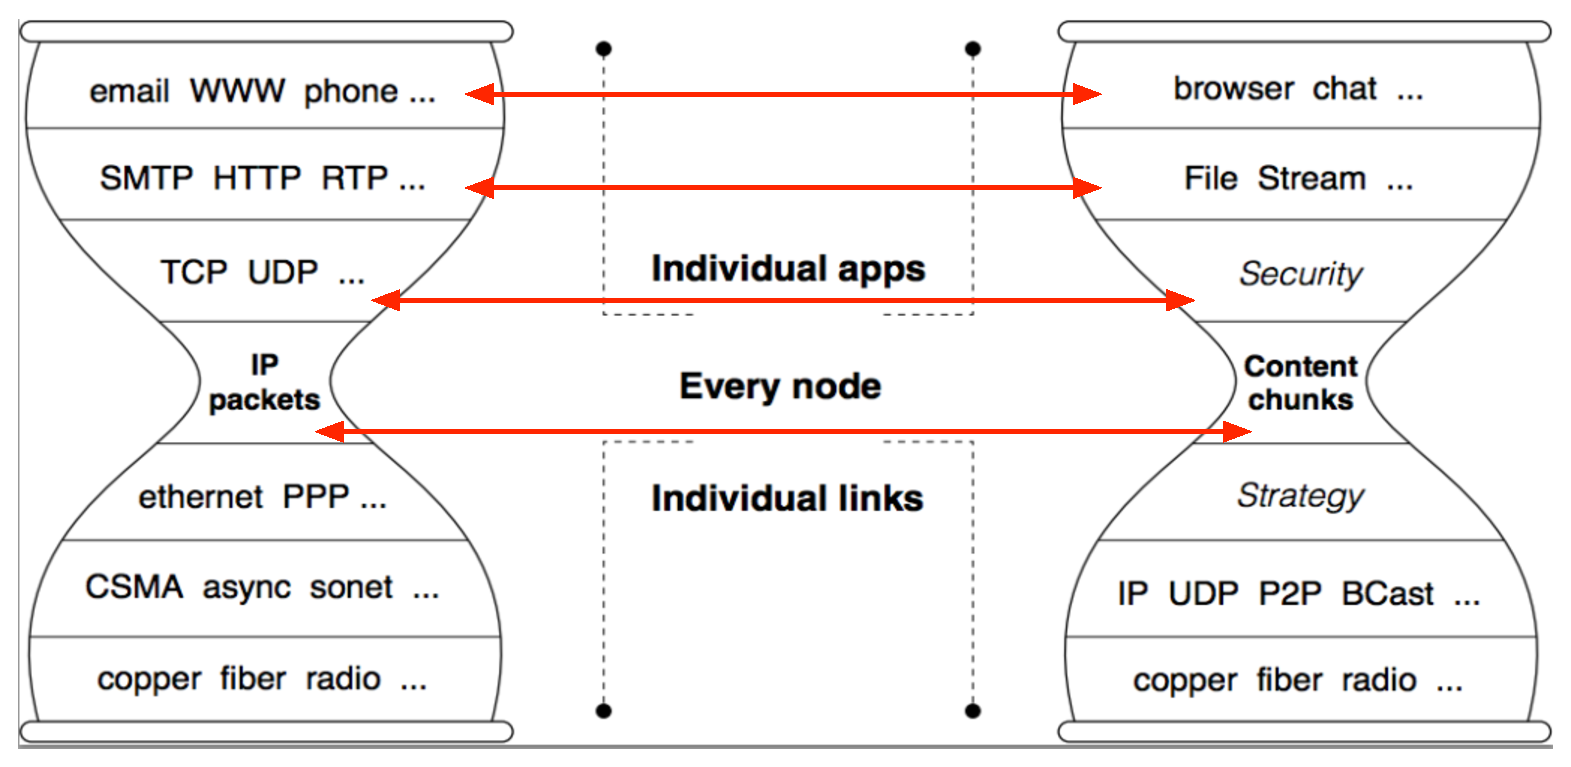
\includegraphics[scale=0.5]{./images/hourglass_conn.pdf}
\label{fig:hourglass}
\caption{TODO}
\end{center}
\end{figure}

The gateway middleware is designed so as to support bi-directional traffic flowing from both types of networks. In what follows we describe how traffic in both directions will be supported internally by the gateway.

\subsection{IP-to-NDN Traffic}
TODO

\subsection{NDN-to-IP Traffic}
TODO

%%%%%%%%%%%%%%%%%%%%%
%%% END MAIN CONTENT
%%%%%%%%%%%%%%%%%%%%%

%%% BIBLIOGRAPHY
\begin{thebibliography}{[MT1]}

\bibitem{first} V. Jacobson, D. K. Smetters, J. D. Thornton, M. F. Plass, N. H. Briggs, R. L. Braynard (PARC) Networking Named Content, CoNEXT 2009, Rome, December, 2009.

\bibitem{NDNtech} L. Zhang, D. Estrin, J. Burke, V. Jacobson, J. D. Thornton, D. K. Smetters, B. Zhang, G. Tsudik, K.C. Claffy, D. Krioukov, D. Massey, C. Papadopoulos, T. Abdelzaher, L. Wang, P. Crowley, and E. Yeh. Named Data Networking (NDN) Project. PARC Tech Report 2010-003, NDN-0001 (2010).

\bibitem{ccnx} Content Centric Networking (CCNx) - Project CCNx. Available online at: \url{https://github.com/ProjectCCNx/ccnx}. Last accessed: 4/2/14.

\end{thebibliography}

\end{document}
